\section{An Illustrative Example}
\label{illustrative-example}


%% Loading and unloading costs no fuel, while driving costs between 1 and
%% 5 fuels units (as indicated by edge labels).\\ The amount of fuel
%% available is 1.5 times higher than needed to deliver all packages;
%% concretely, the initial fuel in trucks is $fuel(T_0) = 16$, $fuel(T_1)
%% = 7$.

To illustrate our approach and the kind of answers it provides to user
questions, let us briefly consider the IPC NoMystery domain, a
classical transportation domain with fuel
consumption. Figure~\ref{fig:nomystery-example} illustrates an example
instance with two trucks and three packages. Fuel costs are indicated
at road segments (initial fuel is $16$ for $T_0$ and $7$ for
$T_1$). All packages are initially at $L_0$ (shown in blue); they need
to be delivered to individual goal locations (shown in red).

\begin{wrapfigure}{r}{0.5\columnwidth}
\vspace{-0.4cm} \hspace{-0.4cm} 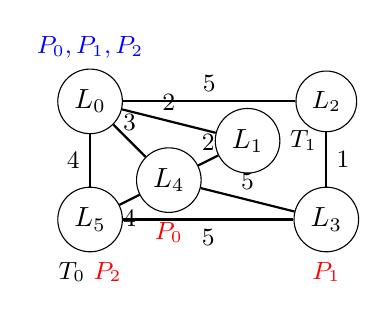
\begin{tikzpicture}[scale=0.5]
  \node[draw, circle, label=above:{\small \textcolor{blue}{$P_0, P_1,P_2$}}] (l0) at (0,0) {$L_0$};
  \node[draw, circle, label=right:{\small $T_1$}] (l1) at (4,-1) {$L_1$};
  \node[draw, circle] (l2) at (6,0) {\small $L_2$};
  \node[draw, circle, label=below:{\small \textcolor{red}{$P_1$}}] (l3) at (6,-3) {$L_3$};
  \node[draw, circle, label=below:{\small \textcolor{red}{$P_0$}}] (l4) at (2,-2) {$L_4$};
  \node[draw, circle, label=below:{\small $T_0$ \textcolor{red}{$P_2$}}] (l5) at (0,-3) {$L_5$};

  \draw[thick] (l0) to node[above] {\small 5} (l2);
  \draw[thick] (l0) to node[above] {\small 2} (l1);
  \draw[thick] (l0) to node[above] {\small 3} (l4);
  \draw[thick] (l0) to node[left] {\small 4} (l5);
  \draw[thick] (l2) to node[right] {\small 1} (l3);
  \draw[thick] (l4) to node[above] {\small 2} (l1);
  \draw[thick] (l4) to node[above] {\small 5} (l3);
  \draw[thick] (l5) to node[below] {\small 5} (l3);
  \draw[thick] (l4) to node[below] {\small 4} (l5);
\end{tikzpicture}
\vspace{-0.2cm}
\hspace{-0.6cm} \caption{Illustrative IPC NoMystery example.}
\label{fig:nomystery-example}
\vspace{-0.2cm}
\end{wrapfigure}

We define three kinds of action-set properties for this domain:
\emph{uses $T_i$ $(L_x,L_y)$} (truck $T_i$ drives at least once from
$L_x$ to $L_y$ or vice versa); \emph{doesn't use $T_i$ $(L_x,L_y)$}
(truck $T_i$ does not drive from $L_x$ to $L_y$ or vice versa);
\emph{same truck $P_x$ $P_y$} (both packages are delivered by the same
truck). We consider six instances of these properties: 1.\ uses $T_0$
$(L_2,L_3)$; 2.\ same truck $P_1$ $P_2$; 3.\ uses $T_0$ $(L_4,L_3)$;
4.\ same truck $P_2$ $P_0$; 5.\ doesn't use $T_0$ $(L_0,L_5)$;
6.\ uses $T_1$ $(L_5,L_4)$.

Fixing the package destinations as hard goals (defining the set of
plans \plans\ considered), and computing the MUGS over these six
action-set properties using the algorithms previously described, it
turns out there are 7 minimal unsolvable subsets of these properties,
each of size 3.

Say now that the current plan uses $T_0$ only, and includes the action
(drive T0 L5 L0). The user might ask \emph{''Why don't you avoid the
  road $L_0-L_5$, which has a lot of traffic at the
  moment?''}. Answering this question in terms of contrastive
explanation, as previously discussed, corresponds to forcing property
5 to be satisfied. At the same time, the plan already satisfies
properties 2 and 4. However, one of the MUGS is $\{2,4,5\}$, and hence
the answer to the user question would be: \textit{Because if you don't
  use that road, then you would not be able to deliver all packages
  using a single truck}.
